%% The following is a directive for TeXShop to indicate the main file
%%!TEX root = report.tex

\chapter{Results}
\label{ch:Results}

\section{Test Hardware}

The primary system for testing was provided by Intel Research; this was physical hardware
and I had console level access to the system --- in fact, I reinstalled Fedora on the
system at one point.  My own test runs collected data on the system configuration.  I
capture that information here.

The Linux version (notably the kernel) was a current version at the time of testing:

\begin{verbatim}
# uname -a
  Linux intelsdp1044 4.17.12-200.fc28.x86_64 #1 \
  SMP Fri Aug 3 15:01:13 UTC 2018 x86_64 x86_64 \
  x86_64 GNU/Linux
\end{verbatim}

It included support for NVM as part of the base release package --- this was \textit{not}
a custom build.

The CPU information for the system is described in Tables \ref{table:results:hardware} \& \ref{table:results:hardware:2}.

\begin{table}
    \caption{Hardware Configuration Information (\textbf{lscpu}) Part 1}\label{table:results:hardware}
    \begin{tabular}{@{}cl@{}}
        Characteristic & Value  \\ \toprule
        Architecture &  x86\_64 \\
        CPU op-mode(s)&      32-bit, 64-bit \\
        Byte Order&          Little Endian \\
        CPU(s)&              96 \\
        On-line CPU(s) list& 0-95 \\
        Thread(s) per core&  2 \\
        Core(s) per socket&  24 \\
        Socket(s)&           2 \\
        NUMA node(s)&        2 \\
        Vendor ID&           GenuineIntel \\
        CPU family&          6 \\ 
        Model&               85 \\ 
        Model name&          Genuine Intel(R) CPU 0000\%@ \\
        Stepping&            5 \\
        CPU MHz&             2899.999 \\
        CPU max MHz&         3700.0000 \\
        CPU min MHz&         1000.0000 \\
        BogoMIPS&            4400.00 \\
        Virtualization&      VT-x \\
        L1d cache&           32K \\
        L1i cache&           32K \\
        L2 cache&            1024K \\
        L3 cache&            33792K \\
        NUMA node0 CPU(s)&   0-23,48-71 \\
        NUMA node1 CPU(s)&   24-47,72-95 \\
        \bottomrule
    \end{tabular}%
\end{table}

\begin{table}
        \caption{Hardware Configuration Information (\textbf{lscpu}) Part 2}\label{table:results:hardware:2}
        \begin{tabular}{@{}cl@{}}
        Flags & fpu vme de pse tsc msr pae mce cx8 apic sep \\
        & mtrr pge mca cmov pat pse36 clflush dts acpi \\
        & mmx fxsr sse sse2 ss ht tm pbe syscall nx pdpe1gb \\
        & rdtscp lm constant\_tsc art arch\_perfmon pebs \\
        & bts rep\_good nopl xtopology nonstop\_tsc cpuid \\
        & aperfmperf pni pclmulqdq dtes64 monitor ds\_cpl vmx \\
        & smx est tm2 ssse3 sdbg fma cx16 xtpr pdcm pcid dca \\
        & sse4\_1 sse4\_2 x2apic movbe popcnt aes xsave avx \\
        & f16c rdrand lahf\_lm abm 3dnowprefetch cpuid\_fault \\
        & epb cat\_l3 cdp\_l3 invpcid\_single pti intel\_ppin \\
        & mba ibrs ibpb stibp tpr\_shadow vnmi flexpriority \\
        & ept vpid fsgsbase tsc\_adjust bmi1 hle avx2 smep \\
        & bmi2 erms invpcid rtm cqm mpx rdt\_a avx512f \\ 
        & avx512dq rdseed adx smap clflushopt clwb intel\_pt \\
        & avx512cd avx512bw avx512vl xsaveopt xsavec xgetbv1 \\
        & xsaves cqm\_llc cqm\_occup\_llc cqm\_mbm\_total \\
        & cqm\_mbm\_local dtherm ida arat pln pts hwp \\
        & hwp\_act\_window hwp\_epp hwp\_pkg\_req pku ospke \\
        \bottomrule
    \end{tabular}%
\end{table}

Memory in the system consisted of 12 32GB DRAM modules and 12 249GB NVM modules.  This information
was displayed using the \verb+dmidecode --type 17+ to display information specific to the memory
modules installed on the machine.

DRAM modules appeared like:

\begin{verbatim}
    Handle 0x0026, DMI type 17, 40 bytes
Memory Device
	Array Handle: 0x0024
	Error Information Handle: Not Provided
	Total Width: 72 bits
	Data Width: 64 bits
	Size: 32 GB
	Form Factor: DIMM
	Set: None
	Locator: CPU1_DIMM_A1
	Bank Locator: NODE 1
	Type: DDR4
	Type Detail: Synchronous
	Speed: 2666 MT/s
	Manufacturer: Micron
	Serial Number: 18B132B8
	Asset Tag:  
	Part Number: 36ASF4G72PZ-2G6H1   
	Rank: 2
	Configured Clock Speed: 2666 MT/s
	Minimum Voltage: 1.2 V
	Maximum Voltage: 1.2 V
	Configured Voltage: 1.2 V
\end{verbatim}

NVM modules appeared like:

\begin{verbatim}
    Handle 0x0028, DMI type 17, 40 bytes
Memory Device
	Array Handle: 0x0024
	Error Information Handle: Not Provided
	Total Width: 72 bits
	Data Width: 64 bits
	Size: 255680 MB
	Form Factor: DIMM
	Set: None
	Locator: CPU1_DIMM_A2
	Bank Locator: NODE 1
	Type: DDR4
	Type Detail: Synchronous Non-Volatile
	Speed: 2666 MT/s
	Manufacturer: Intel
	Serial Number: 00000310
	Asset Tag:  
	Part Number: 8089A2173800000310  
	Rank: 1
	Configured Clock Speed: 2666 MT/s
	Minimum Voltage: 1.2 V
	Maximum Voltage: 1.2 V
	Configured Voltage: 1.2 V
\end{verbatim}

I have omitted all but the first instance of each for the sake of brevity; full logs are
available.

Similarly, using the \verb+lshw+ command in Linux, I captured detailed information about 
the system.  The following is the summary information about all memory installed in the
system:

\begin{verbatim}
    *-memory
    description: System Memory
    physical id: 24
    slot: System board or motherboard
    size: 3380GiB
    capabilities: ecc
    configuration: errordetection=ecc
\end{verbatim}

Similarly, this is the information about the first DIMM module:

\begin{verbatim}
  *-bank:0
       description: DIMM DDR4 Synchronous 2666 MHz (0.4 ns)
       product: 36ASF4G72PZ-2G6H1
       vendor: Micron
       physical id: 0
       serial: 18B132B8
       slot: CPU1_DIMM_A1
       size: 32GiB
       width: 64 bits
       clock: 2666MHz (0.4ns)
\end{verbatim}

Note that this provides different, but consistent information.  For example, the
serial numbers match between the two commands.

The NVM information:

\begin{verbatim}
  *-bank:1
       description: DIMM DDR4 Synchronous Non-volatile 2666 MHz (0.4 ns)
       product: 8089A2173800000310
       vendor: Intel
       physical id: 1
       serial: 00000310
       slot: CPU1_DIMM_A2
       size: 249GiB
       width: 64 bits
       clock: 2666MHz (0.4ns)
\end{verbatim}

Again, further information has been omitted but is available.

Only three of the NVM modules were provisioned: two for node 0, one for node 1.  These were
\acs{DAX} enabled, with xfs formatted for two of them, and ext4 for one of them.

\begin{verbatim}
# mount
/dev/pmem0 on /mnt/pmem0p1 type xfs (rw,relatime,seclabel,attr2,dax,inode64,noquota)
/dev/pmem2 on /mnt/pmem2 type ext4 (rw,relatime,seclabel,dax)
/dev/pmem10 on /mnt/pmem10 type xfs (rw,relatime,seclabel,attr2,dax,inode64,noquota)
\end{verbatim}

\textit{Note: I have omitted the non-\acs{DAX} volumes here.}  All three were mounted in \acs{DAX}
mode, ensuring that memory mapped files within those file systems were directly accessed by the
test application.

The \verb+ndctl+ command was used to capture information about the NVM provisioning as well:

\begin{verbatim}
    ndctl list --namespaces  --human
    [
      {
        "dev":"namespace0.0",
        "mode":"fsdax",
        "map":"dev",
        "size":"245.11 GiB (263.18 GB)",
        "uuid":"f05281b4-dfa7-4f48-ab8b-41d1f54205aa",
        "raw_uuid":"c6c12d35-853d-418a-8602-846d3fd6091c",
        "sector_size":512,
        "blockdev":"pmem0",
        "numa_node":0
      },
      {
        "dev":"namespace2.0",
        "mode":"fsdax",
        "map":"dev",
        "size":"245.11 GiB (263.18 GB)",
        "uuid":"44071681-9ffa-4df4-bd51-7c51092a83e4",
        "raw_uuid":"ee045c93-52e0-4d5e-9670-7bc82ce691d6",
        "sector_size":512,
        "blockdev":"pmem2",
        "numa_node":0
      },
      {
        "dev":"namespace10.0",
        "mode":"fsdax",
        "map":"dev",
        "size":"245.11 GiB (263.18 GB)",
        "uuid":"a755e8a2-c6ad-426f-8841-cf393bc2b4f9",
        "raw_uuid":"2f6e6311-7a52-4fc3-ac97-763454d18370",
        "sector_size":512,
        "blockdev":"pmem10",
        "numa_node":1
      }
    ]
\end{verbatim}

None of the NVM modules are striped (a potential configuration done via a software striping driver in Linux)
and the sizes correspond to NVM in a single DIMM location.

Finally, I used the \verb+ipmctl+ utility, which is available as part of the various Linux releases (including
Fedora 28, which I used).  It is the \textit{Intel persistent memory control} application.

\begin{verbatim}
# ipmctl show -topology
DimmID	MemoryType	Capacity	PhysicalID	DeviceLocator
0x0001	DCPMEM		249.6 GiB	0x0028		CPU1_DIMM_A2
0x0011	DCPMEM		249.6 GiB	0x002c		CPU1_DIMM_B2
0x0021	DCPMEM		249.6 GiB	0x0030		CPU1_DIMM_C2
0x0101	DCPMEM		249.6 GiB	0x0036		CPU1_DIMM_D2
0x0111	DCPMEM		249.6 GiB	0x003a		CPU1_DIMM_E2
0x0121	DCPMEM		249.6 GiB	0x003e		CPU1_DIMM_F2
0x1011	DCPMEM		249.6 GiB	0x0048		CPU2_DIMM_B2
0x1021	DCPMEM		249.6 GiB	0x004c		CPU2_DIMM_C2
0x1001	DCPMEM		249.6 GiB	0x0044		CPU2_DIMM_A2
0x1111	DCPMEM		249.6 GiB	0x0056		CPU2_DIMM_E2
0x1121	DCPMEM		249.6 GiB	0x005a		CPU2_DIMM_F2
0x1101	DCPMEM		249.6 GiB	0x0052		CPU2_DIMM_D2
N/A	DDR4		32.0 GiB	0x0026		CPU1_DIMM_A1
N/A	DDR4		32.0 GiB	0x002a		CPU1_DIMM_B1
N/A	DDR4		32.0 GiB	0x002e		CPU1_DIMM_C1
N/A	DDR4		32.0 GiB	0x0034		CPU1_DIMM_D1
N/A	DDR4		32.0 GiB	0x0038		CPU1_DIMM_E1
N/A	DDR4		32.0 GiB	0x003c		CPU1_DIMM_F1
N/A	DDR4		32.0 GiB	0x0042		CPU2_DIMM_A1
N/A	DDR4		32.0 GiB	0x0046		CPU2_DIMM_B1
N/A	DDR4		32.0 GiB	0x004a		CPU2_DIMM_C1
N/A	DDR4		32.0 GiB	0x0050		CPU2_DIMM_D1
N/A	DDR4		32.0 GiB	0x0054		CPU2_DIMM_E1
N/A	DDR4		32.0 GiB	0x0058		CPU2_DIMM_F1
\end{verbatim}

This captures the system configuration in a compact form, demonstrating the full amount of memory on
the test system.


\section{Intel Memory Latency Checker}

The measurements in this section were collected using the Intel Memory Latency Checker, a tool
developed by Intel to evaluate memory bandwidth and latency.  Version 3.5 includes explicit
support for evaluating DRAM and NVM.  It is NUMA aware and can be used for evaluating both
node-local as well as node-remote memories.~\cite{IntelMLC35}

I note that the provided documentation for this tool does not describe some modes of
this tool that are, in fact, used in this evaluation.  Further, actually enabling the
correct testing mode for NVM is not easy to reproduce from the information available.
Thus, when reporting specific results I have included the command line switches used
as part of the testing. 

The tests considered in this section all used a zero injection latency (\texttt{-d0},)
as this represents the highest workload against the given memory --- latency injection
provides a simple mechanism for evaluating performance on workloads that are not
pushing the bandwidth boundary.  While I did perform evaluations with higher
injection rates, I have chosen to omit that additional data from this report.

Each specific test run uses various flags to control the behavior.  Unless
otherwise noted, all tests used the \verb+--loaded_latency+ option, which
means that the test utility is measuring the latency of the memory with
some load imposed.

Note that for all tests, \textbf{core 0} is used for measurements.  Thus, when
we report 3 cores in use, two of them are generating load and one is performing
the latency measurements.

For the various tests I use the switches as shown in Table \ref{mlc:switches}.

\begin{table}
    \caption{MLC switches used during testing}\label{mlc:switches}
    \begin{tabular}{@{}clc@{}}
        Switch & Effect & See Section \\ \toprule
        \verb+-d+ & Latency injection (seconds) &  \\
        \verb+-t+ & Test time (seconds) &  \\
        \verb+-l+ & Stride size (bytes) & \\
        \verb+-R+ & Read-only workload & \ref{baseline:dram}, \ref{baseline:nvm} \\
        \verb+-W2+ & Read-Write 2:1 Workload & \ref{chart:sequential:W2} \ref{chart:random:W2} \\ 
        \verb+-W3+ & Read-Write 3:1 Workload & \ref{chart:sequential:w3} \\
        \verb+-W5+ & Read-Write 1:1 Workload & \ref{chart:random:W5} \ref{chart:sequential:W5} \\
        \verb+-W6+ & Non-Temporal Write Workload & \ref{chart:random:w6} \ref{chart:sequential:W6} \\
        \verb+-W7+ & Read-Non-Temporal-Write 2:1 Workload & \ref{chart:random:W7} \ref{chart:sequential:W7} \\
        \verb+-W8+ & Read-Non-Temporal-Write 1:1 Workload  & \ref{chart:random:W8} \\
        \verb+-W10+ & Read-Non-Temporal-Write 3:1 (Streaming Triad) & \ref{chart:sequential:W10} \\ \bottomrule
    \end{tabular}%
\end{table}

Note that reported stride sizes were 16, 32, 64, 128, 256, 512, 1024, and 2048 in all cases.
In a few cases I report 4096, but for many tests that stride size failed to work properly
with the given test.  Similarly, I tested sizes below 16 bytes but found that it frequently
failed.

\subsection{Sanity Check}

\begin{figure}
    \centering
    \caption{Bandwidth Evaluation of Test System against Intel Reference}\label{chart:aep:bw}
    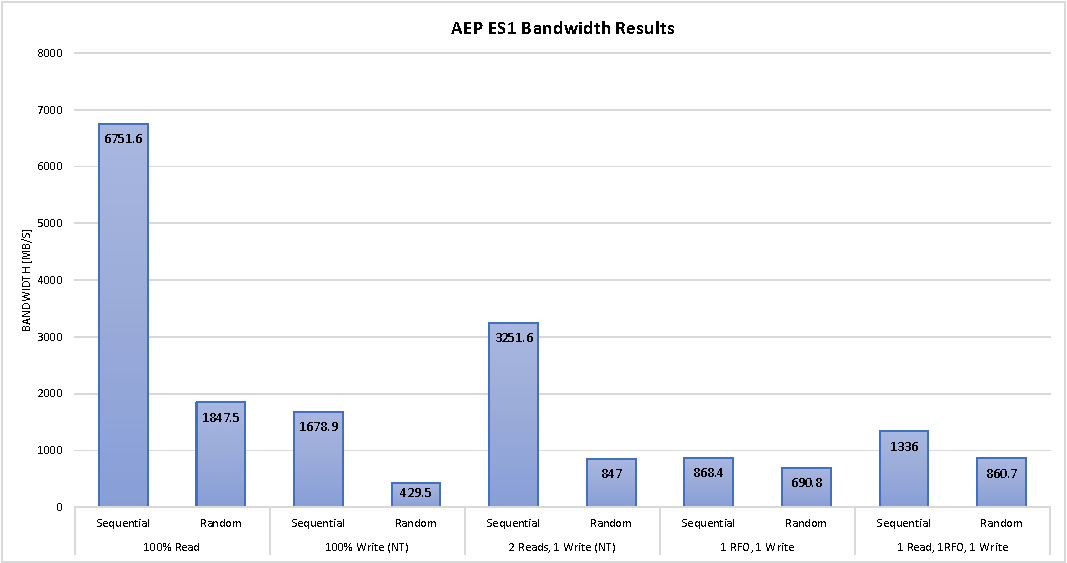
\includegraphics[scale=0.5]{charts/aep_eval_bandwidth-crop.pdf}
\end{figure}

\begin{figure}
    \centering
    \caption{Idle Latency Evaluation of Test System against Intel Reference}\label{chart:aep:idle}
    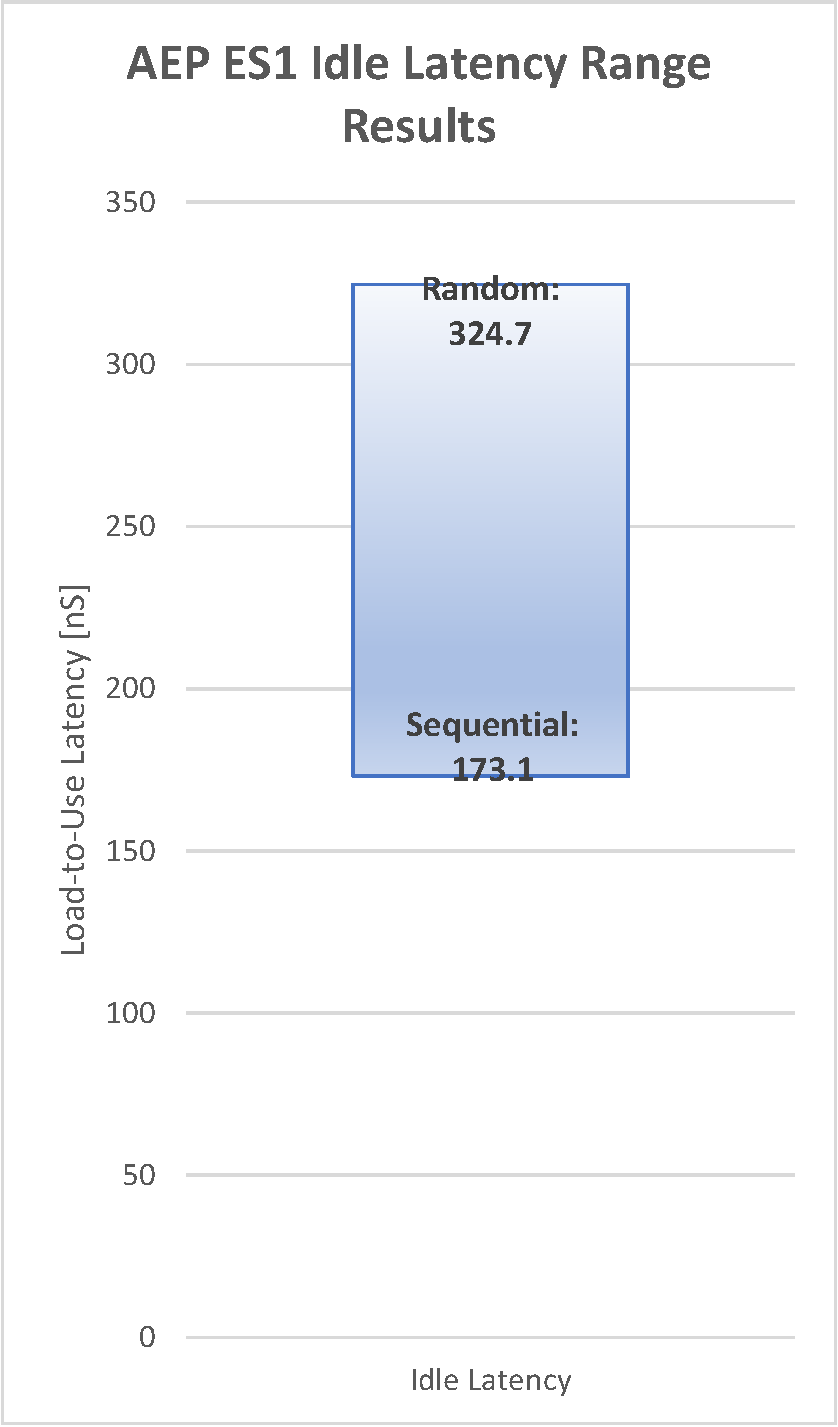
\includegraphics[scale=0.5]{charts/aep_eval_idle_latency-crop.pdf}
\end{figure}

\begin{figure}
    \centering
    \caption{Random Read Load Latency Evaluation of Test System against Intel Reference}\label{chart:aep:read}
    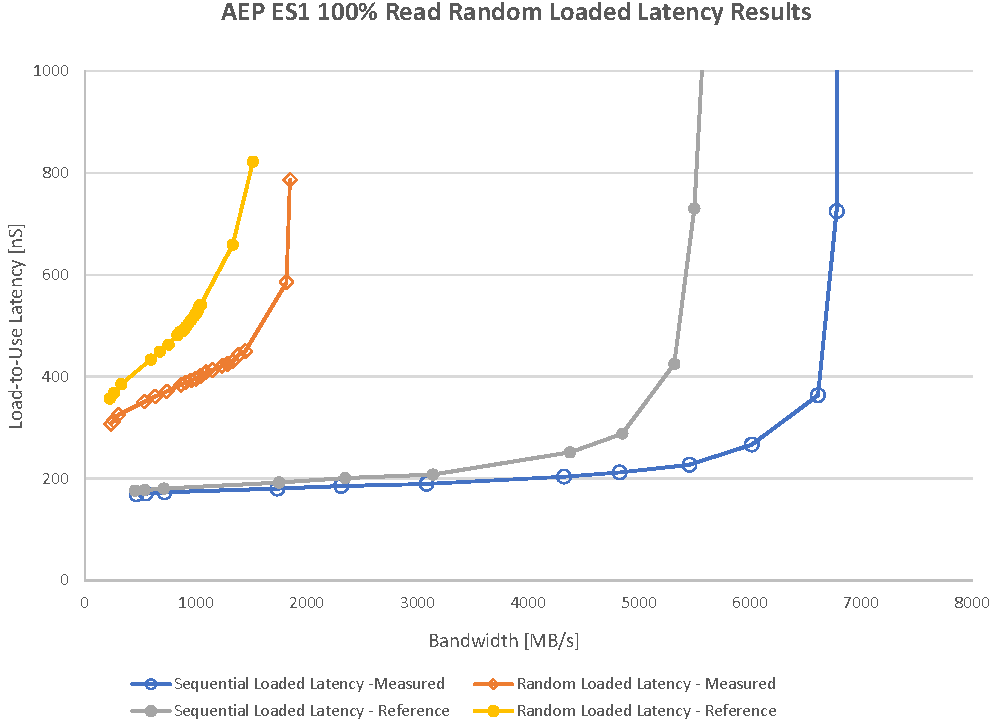
\includegraphics[scale=0.5]{charts/aep_eval_random_read_load_latency-crop.pdf}
\end{figure}

\begin{table}
    \centering
    \caption{Test System versus Intel Reference}\label{mlc:reference}
    \begin{tabular}{@{}cl@{}}
        Test Description & Figure \\ \toprule
        Idle Memory Latency & \ref{chart:aep:idle} \\
        Loaded Memory Bandwidth & \ref{chart:aep:bw} \\
        Random Read Latency & \ref{chart:aep:read} \\ \bottomrule
    \end{tabular}%
\end{table}


Because the early results I was observing were surprising, I spent time to verify that I was
using the tools properly by reproducing the original Intel results.  This exercise was
useful because it allowed me to identify undocumented options being used by Intel in
their own evaluation, understanding how to enable their ``persistent memory'' mode in
the tests, and validate that I was able to obtain comparable results, suggesting that
I was indeed testing the hardware appropriately.  Ultimately, I did adjust my own data
collection techniques to ensure that I was enabling persistent memory mode.

Intel provided benchmark numbers for three tests and the scripts to repeat their tests
on the actual test system. These tests, and the results, are shown in Table \ref{mlc:reference}.
The results were slightly faster, as I was using a newer system, but within 20\% of the original
Intel reference numbers.

\subsection{Non-Temporal Baseline Measurements}


This section describes the information for \textbf{non-temporal move} operations on the same node. Because
these are done as non-temporal move operations, they bypass the cache and write directly to the actual
memory.  Note that the failure domain is discussed in greater detail in \S \ref{section:model:failure}.
The transfer involved here is sufficiently large that the impact of the memory controller caching
does not impact behavior.

\subsubsection{DRAM}\label{baseline:dram}

\begin{figure}
    \centering
    \caption{Baseline Measurement of DRAM Non-Temporal Write on the same NUMA Node}\label{chart:baseline:dram}
    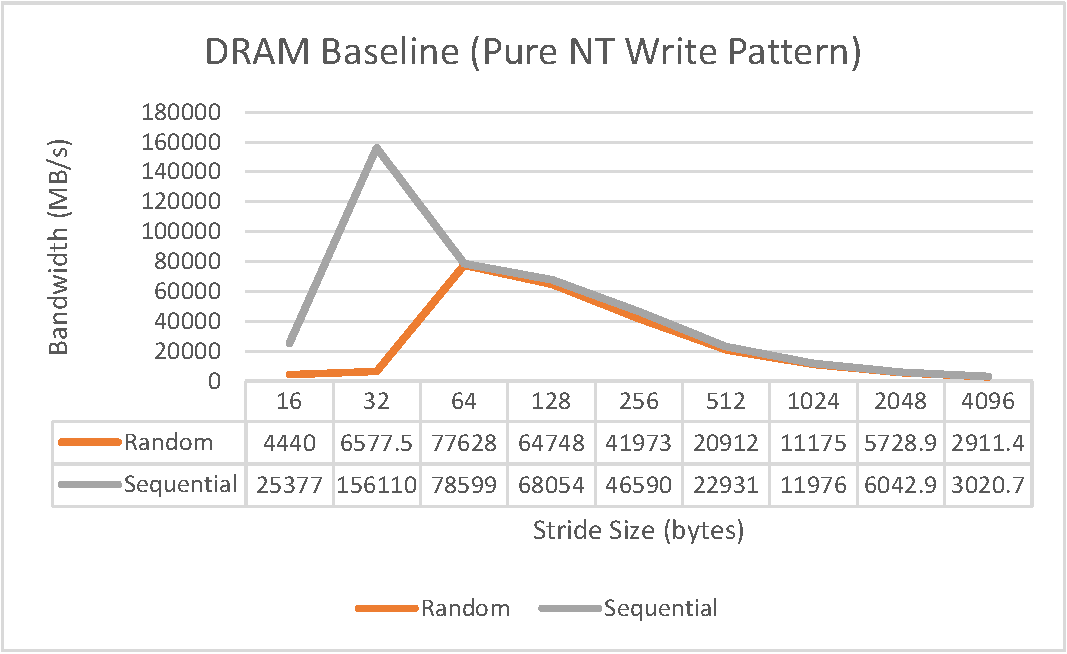
\includegraphics[width=1\textwidth]{charts/dram-baseline-nt-write-same-node-crop.pdf}
\end{figure}

Baseline testing was done using the switches:

\begin{verbatim}
    --loaded_latency -d0 -t10 -W6 -l1024 -T 
        -odata/bw_ctl_pmem0p1_seq_W6-0_23_400000_dram.dat
\end{verbatim}

The file \verb+data/bw_ctl_pmem0p1_seq_W6-0_23_400000_dram.dat+ contained the confirmation information
for the specific test layout:

\begin{verbatim}
0       W6 seq 400000 dram 0
1-23    W6 seq 400000 dram 0
\end{verbatim}

This drives the test to use core 0 for latency measurements, and cores 1-23 for load generation.

Note that the \verb+-l+ option was varied depending upon the ``stride'' size (unit of data handling).
The control file specified the disposition of the individual CPUs

I do not report results for any other DRAM tests.

Results for this test are showin in Figure \ref{chart:baseline:dram}.

\subsubsection{NVM}\label{baseline:nvm}

\begin{figure}[b]
\centering
    \caption{Baseline Measurement of NVM Non-Temporal Write on the same NUMA Node}\label{chart:baseline:nvm}
    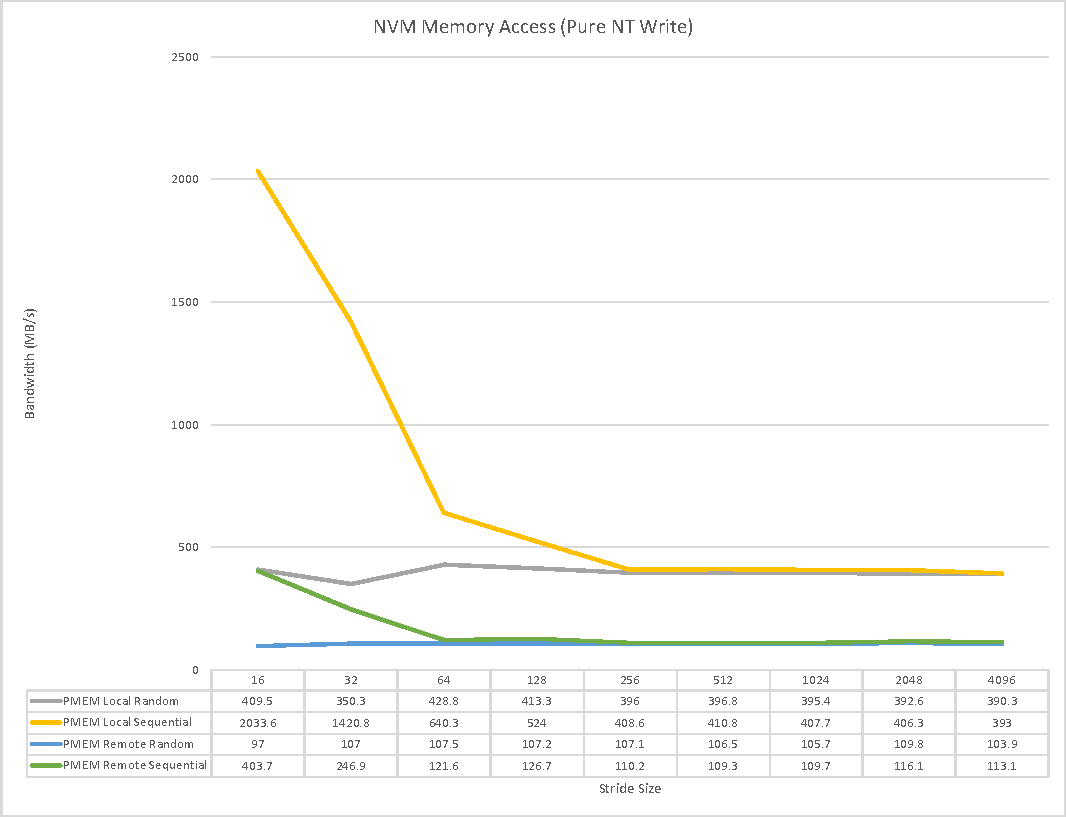
\includegraphics[width=1\textwidth]{charts/nt-write-both-nodes-crop.pdf}
\end{figure}

Baseline testing was done using the switches:

\begin{verbatim}
    --loaded_latency -d0 -t10 -W6 -l64 \
      -odata/bw_ctl_pmem0p1_seq_W6-0_23_400000_pmem.dat}
\end{verbatim}

The file \verb+data/bw_ctl_pmem0p1_seq_W6-0_23_400000_dram.dat+ contained the confirmation information
for the specific test layout:

\begin{verbatim}
0    W6 seq 400000 pmem /mnt/pmem0p1
1-23 W6 seq 400000 pmem /mnt/pmem0p1
\end{verbatim}

The \verb+pmem+ directive is used to put the test utility into ``persistent memory'' testing mode.
The final value is the name of the directory to use.  It \textbf{must} be a persistent memory
to run this test.  Otherwise the test will refuse to run.


\subsection{Cached Read}\label{mlc:r}

\subsubsection{Random Read}
\begin{figure}
    \centering
    \caption{Random Read (R)}\label{chart:random:read}
    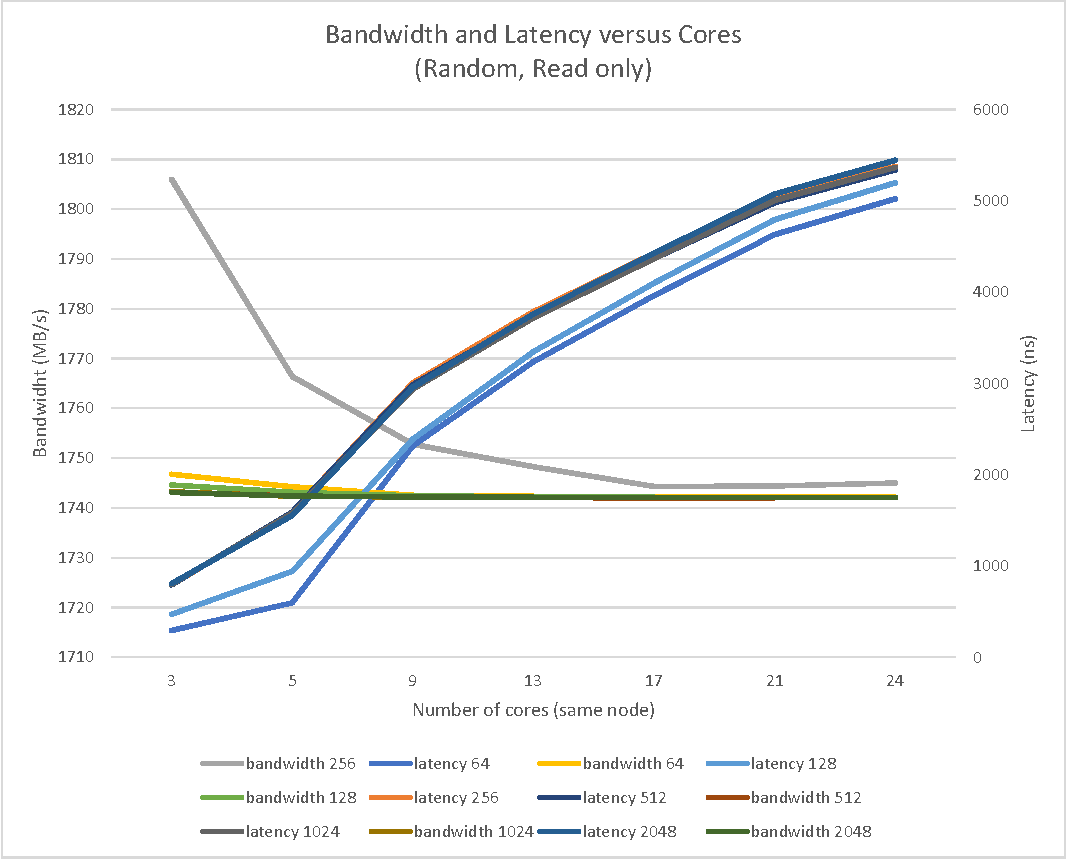
\includegraphics[scale=0.5]{charts/random-r-crop.pdf}
\end{figure}

\begin{figure}
    \centering
    \caption{Sequential Read (R)}\label{chart:sequential:read}
    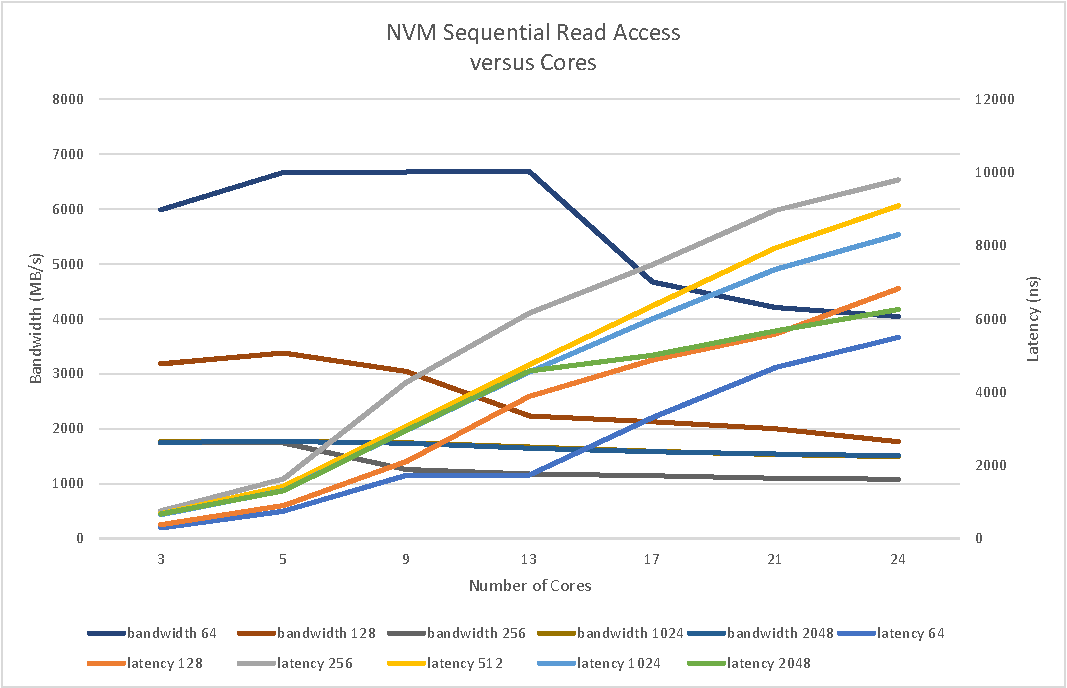
\includegraphics[scale=0.5]{charts/sequential-r-crop.pdf}
\end{figure}

\begin{figure}
    \centering
    \caption{Random 2:1 Read/Write (W2)}\label{chart:random:W2}
    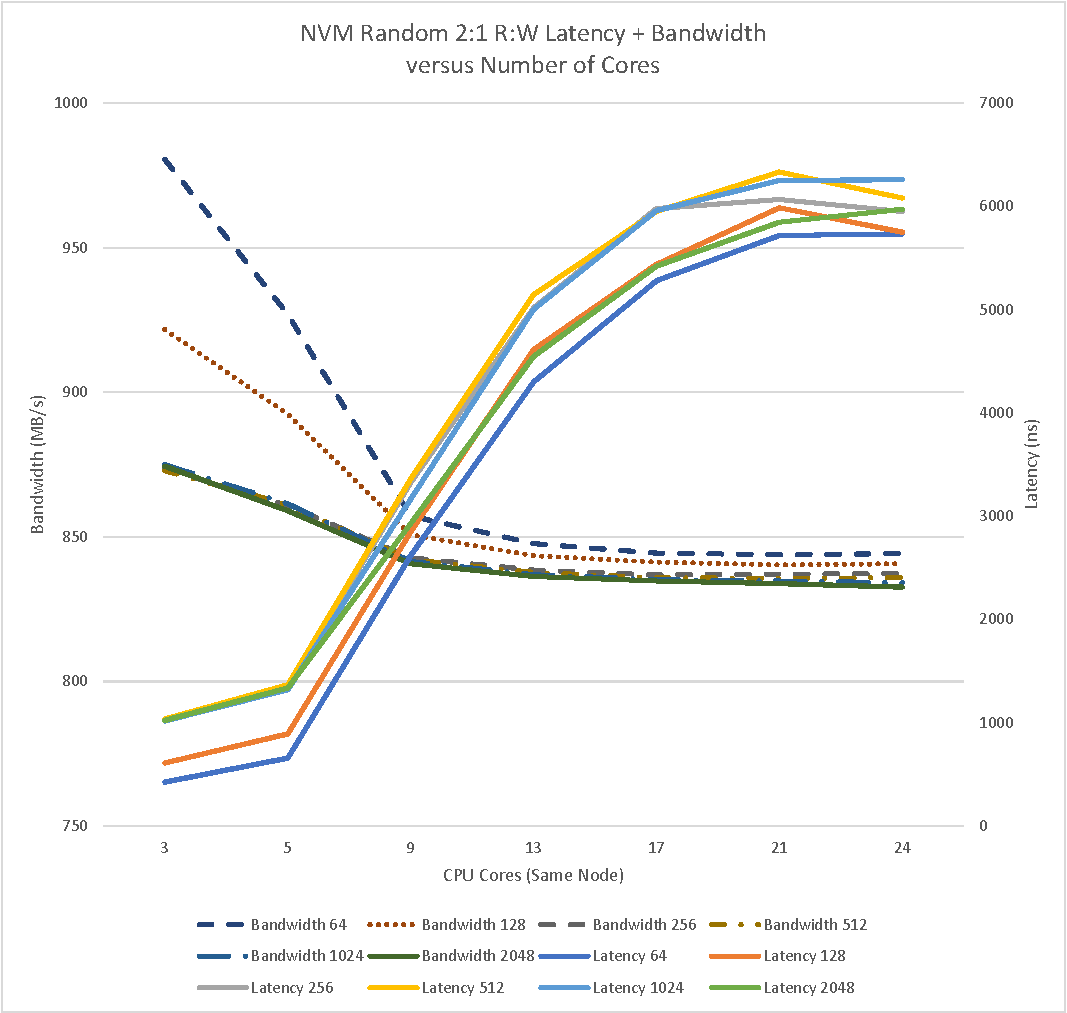
\includegraphics[scale=0.5]{charts/random-w2-crop.pdf}
\end{figure}

\begin{figure}
    \centering
    \caption{Sequential 2:1 Read/Write (W2)}\label{chart:sequential:W2}
    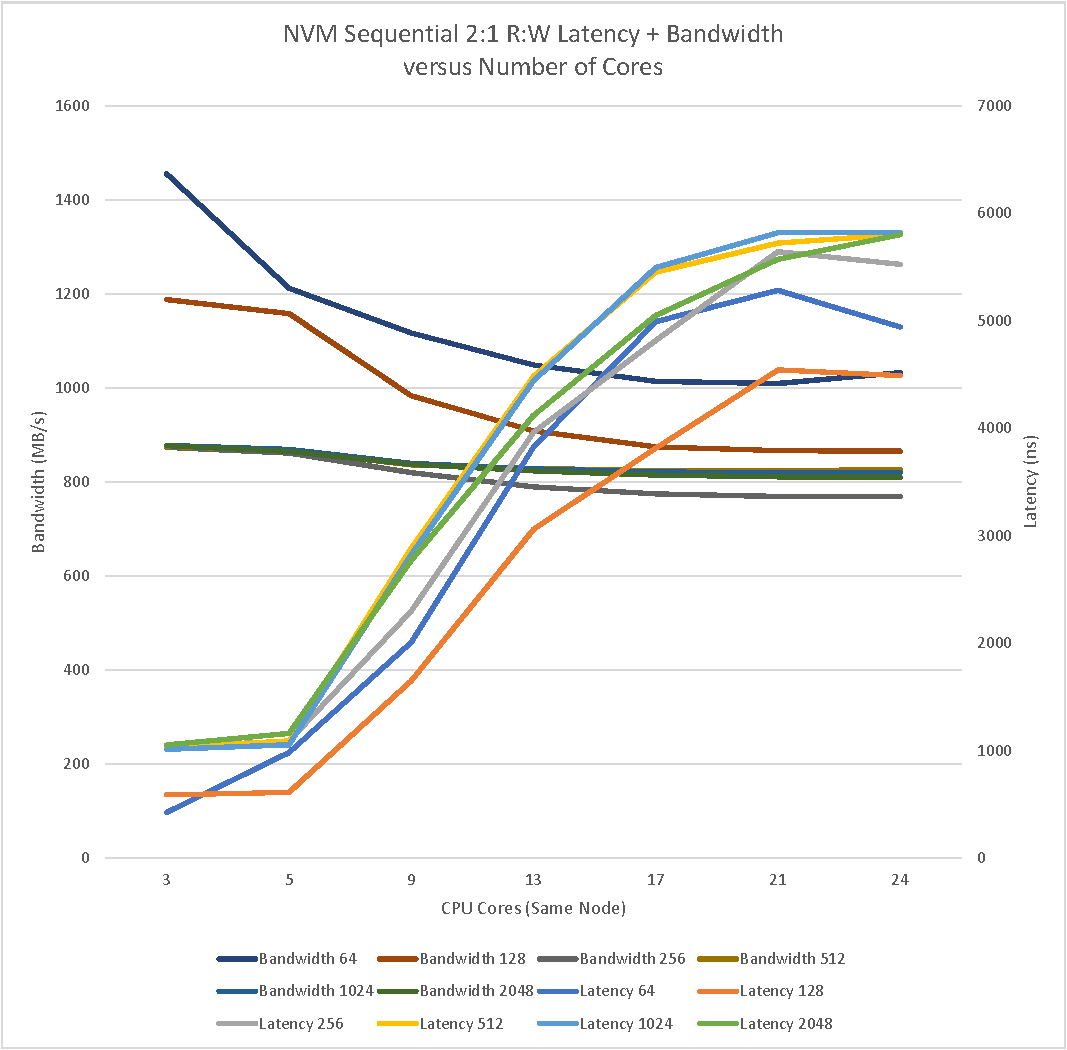
\includegraphics[scale=0.5]{charts/sequential-w2-crop.pdf}
\end{figure}

\begin{figure}
    {\centering
    \caption{Sequential 3:1 Read/Write (W3)}\label{chart:sequential:w3}
    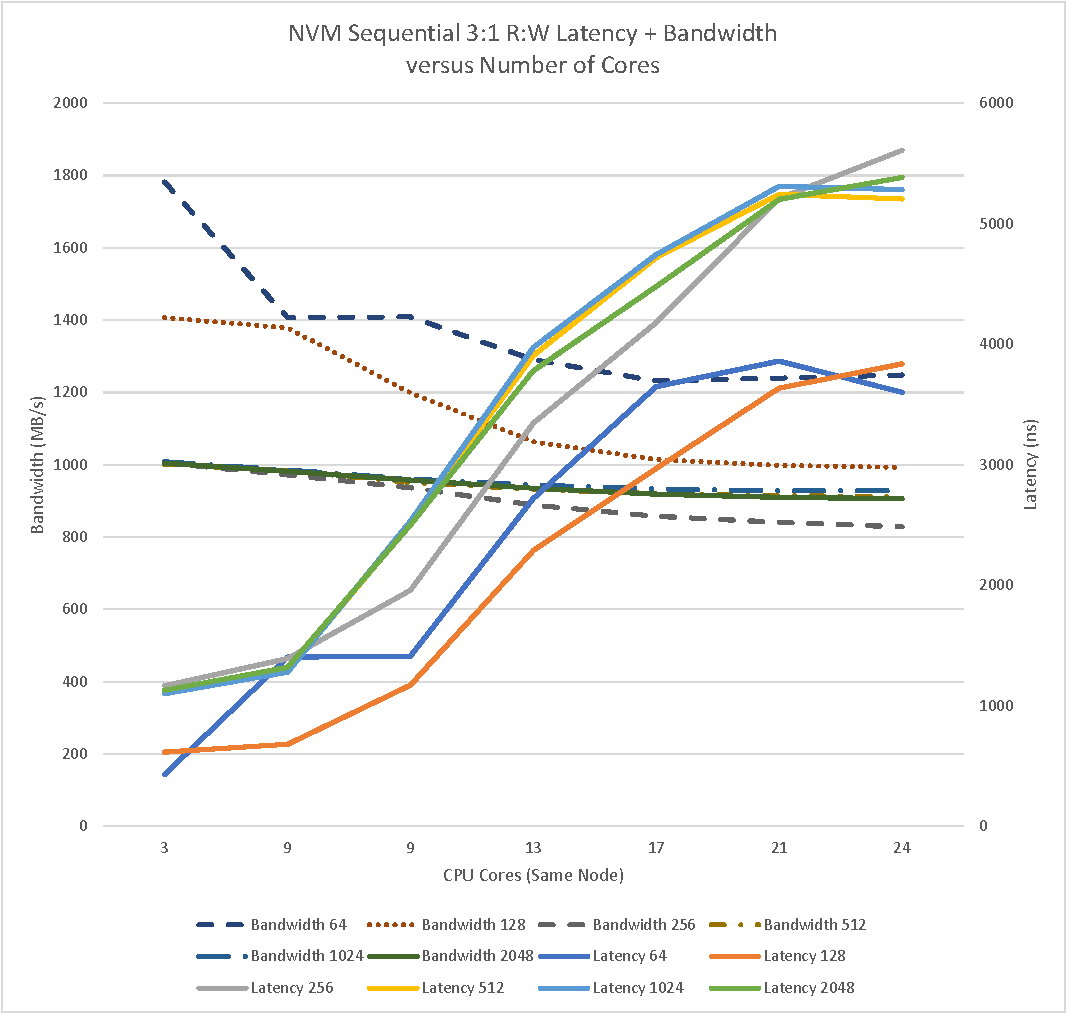
\includegraphics[scale=0.5]{charts/sequential-w3-crop.pdf}
    }
\end{figure}



\begin{figure}
    \centering
    \caption{Random 1:1 Read/Write (W5)}\label{chart:random:W5}
    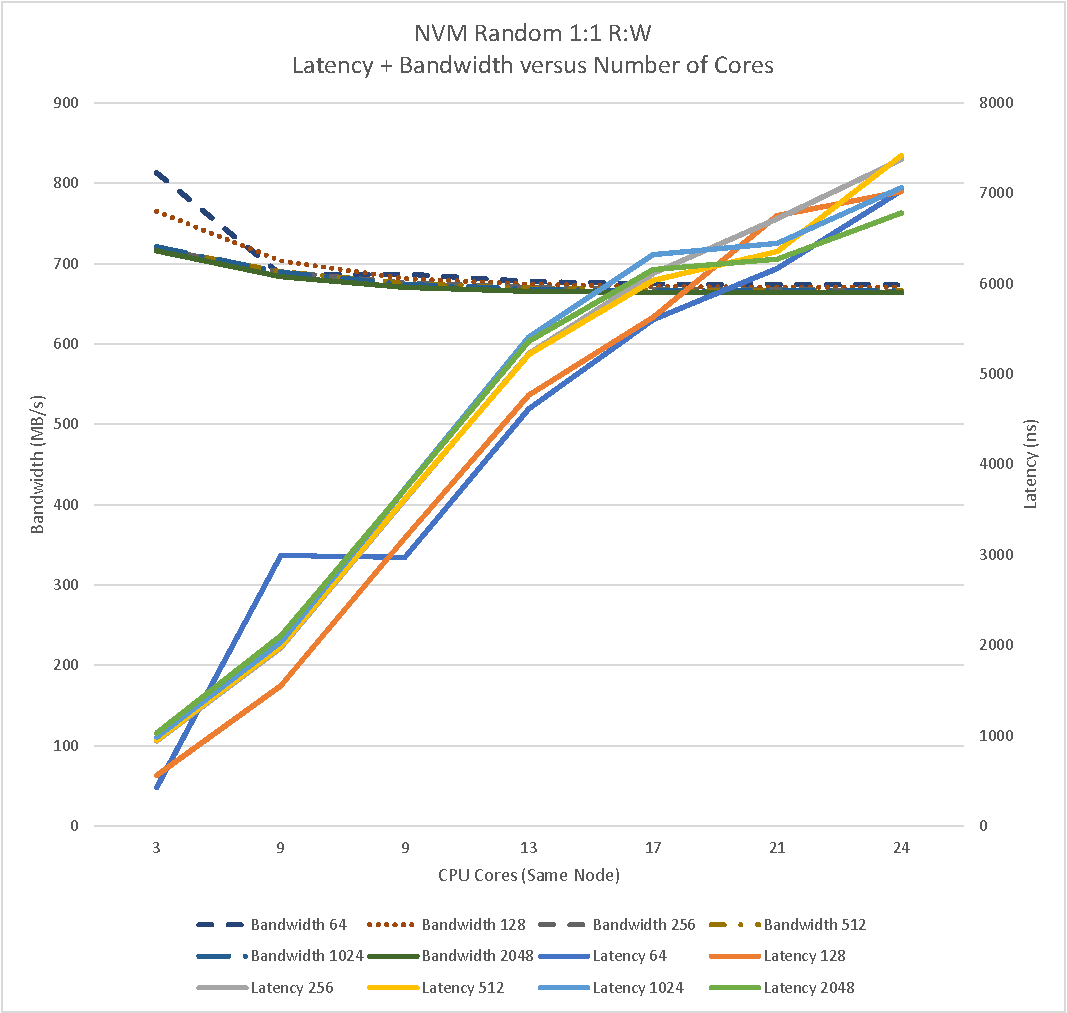
\includegraphics[scale=0.5]{charts/random-w5-crop.pdf}
\end{figure}





\begin{figure}
    \centering
    \caption{Random Non-Temporal Write (W6)}\label{chart:random:w6}
    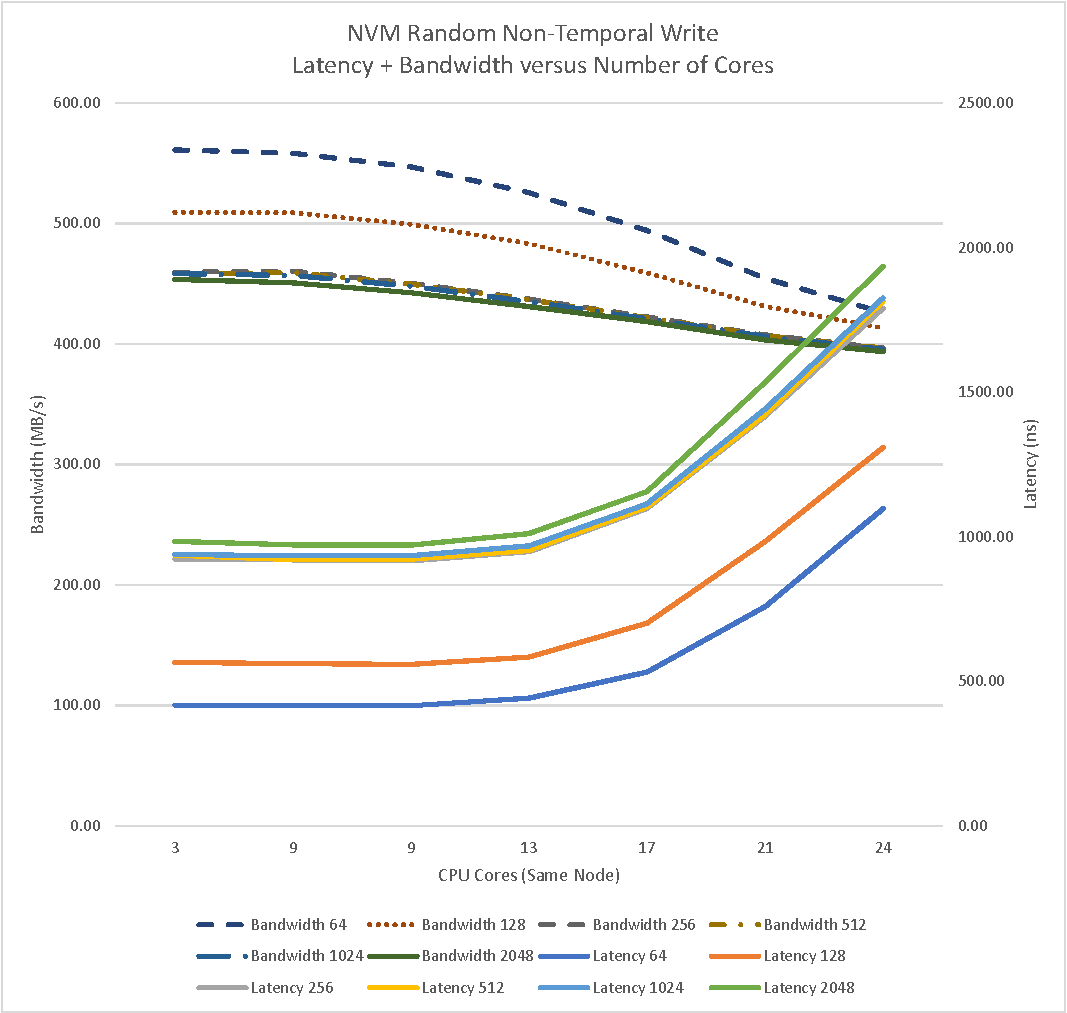
\includegraphics[scale=0.5]{charts/random-w6-crop.pdf}
\end{figure}

\begin{figure}
    \centering
    \caption{Random 2:1 Read to Non-Temporal Write (W7)}\label{chart:random:W7}
    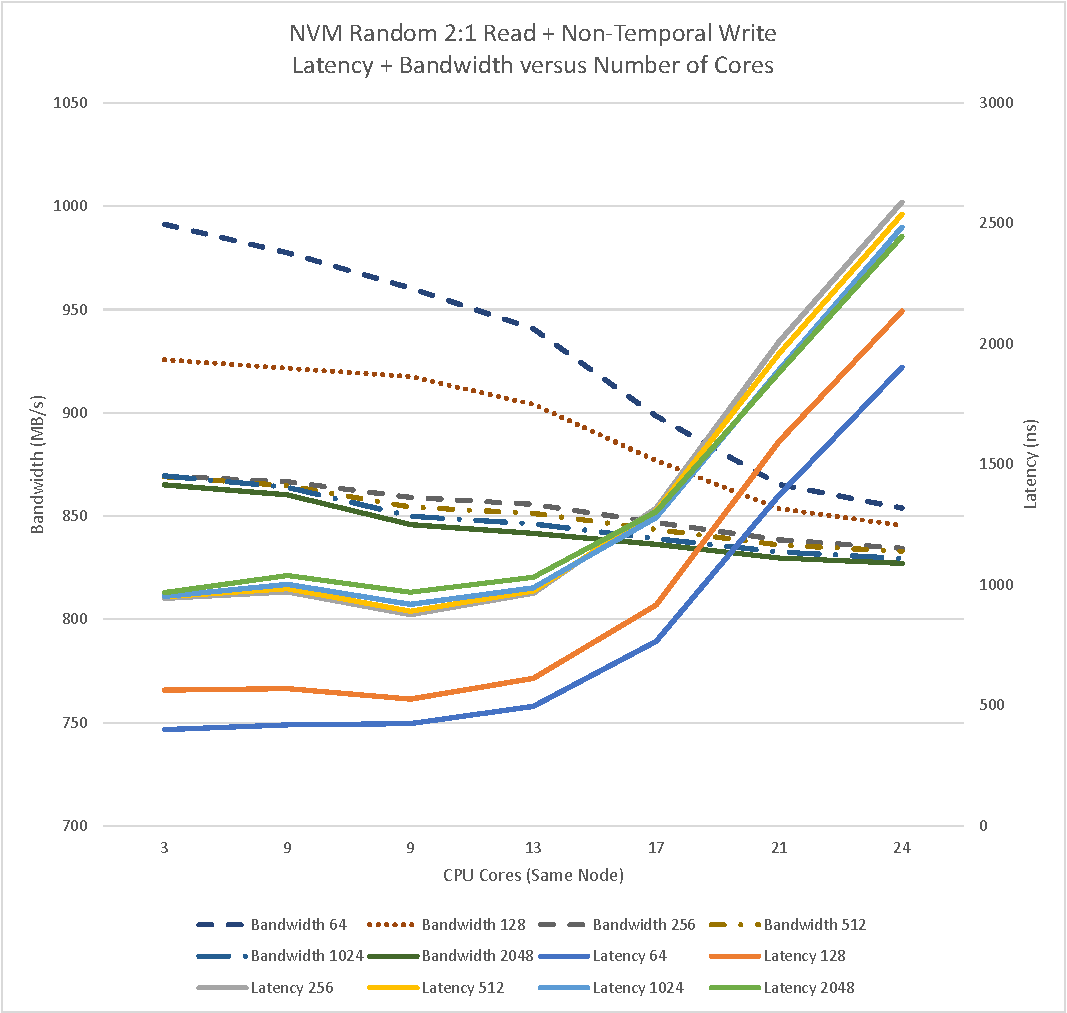
\includegraphics[scale=0.5]{charts/random-w7-crop.pdf}
\end{figure}

\begin{figure}
    \centering
    \caption{Random 1:1 Read to Non-Temporal Write (W8)}\label{chart:random:W8}
    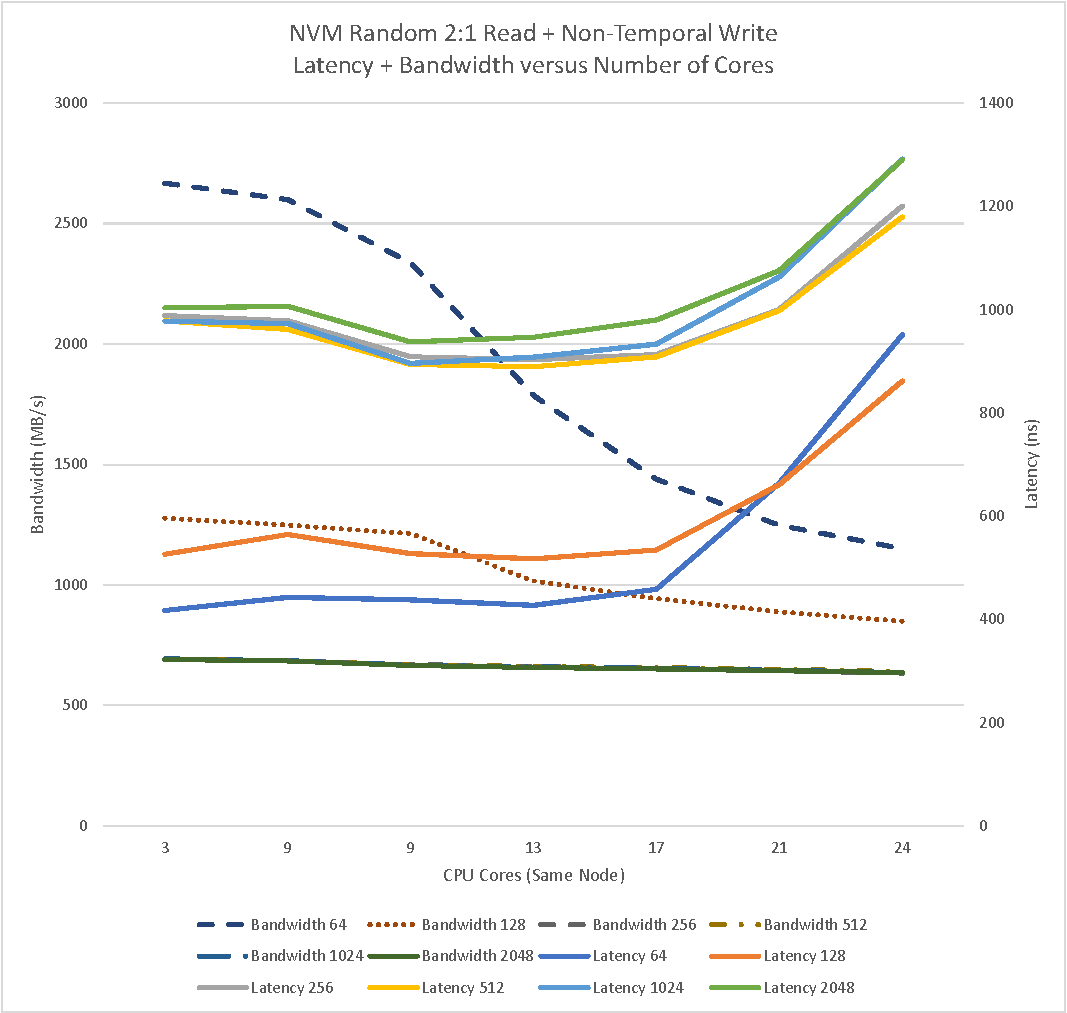
\includegraphics[scale=0.5]{charts/random-w8-crop.pdf}
\end{figure}

\begin{figure}
    \centering
    \caption{Sequential 1:1 Read to Write (W5)}\label{chart:sequential:W5}
    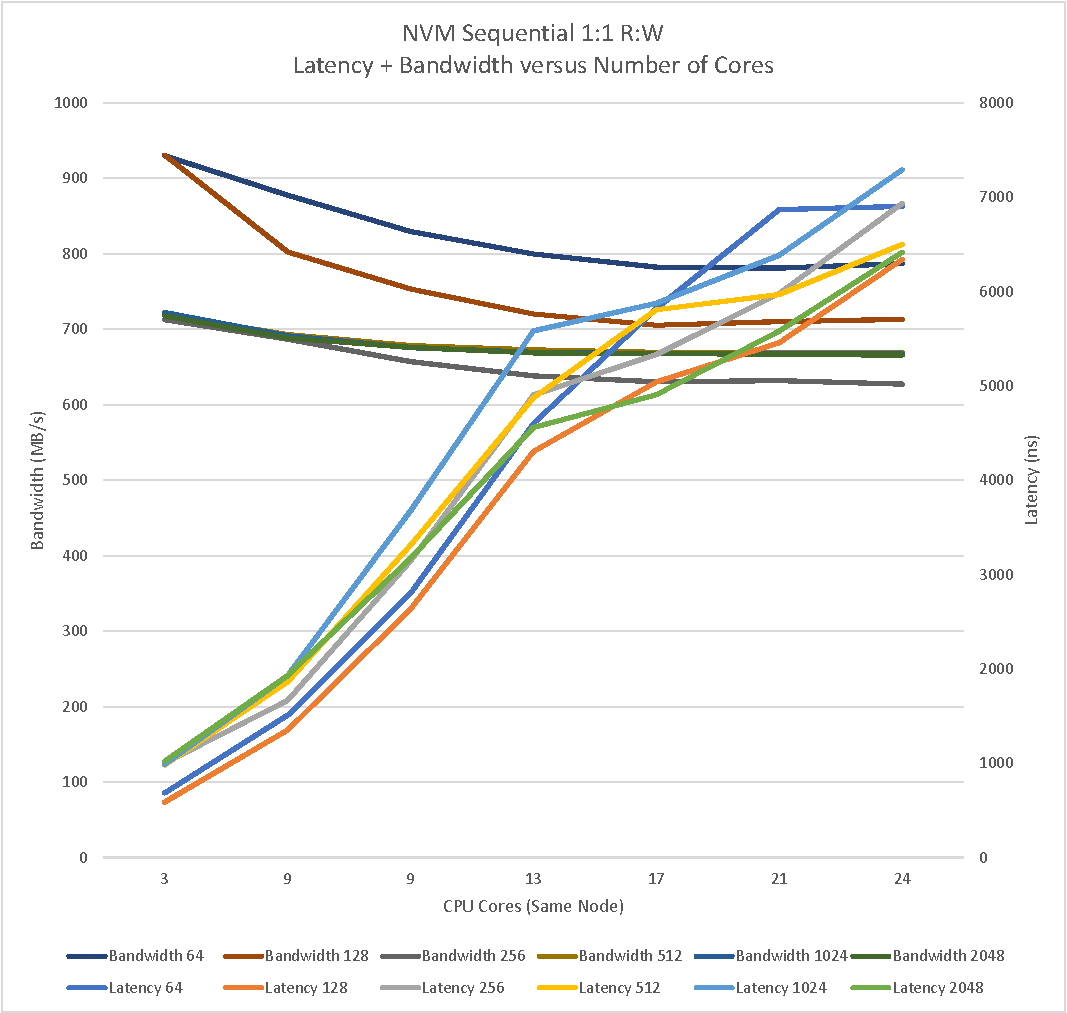
\includegraphics[scale=0.5]{charts/sequential-w5-crop.pdf}
\end{figure}


\begin{figure}
    \centering
    \caption{Sequential Non-Temporal Write (W6)}\label{chart:sequential:W6}
    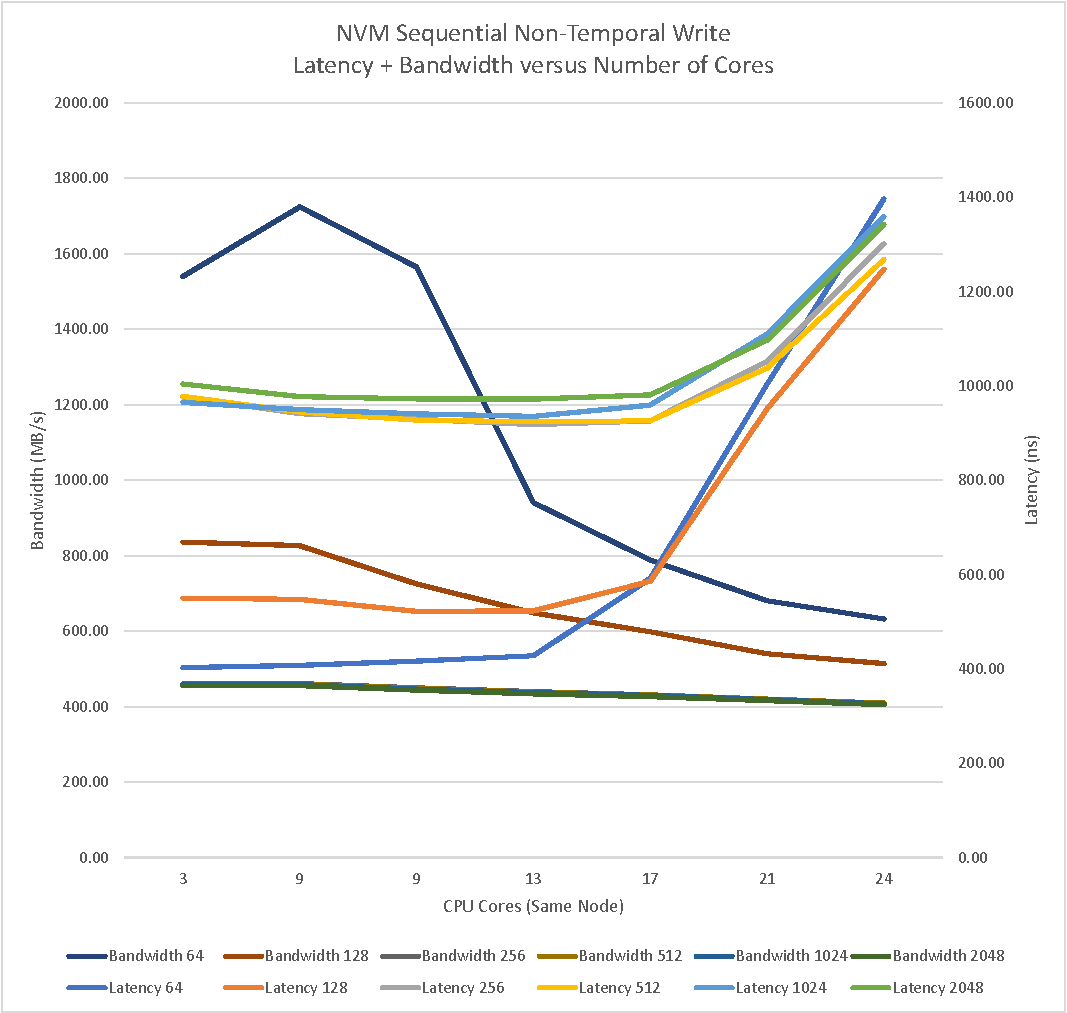
\includegraphics[scale=0.5]{charts/sequential-w6-crop.pdf}
\end{figure}


\begin{figure}
    \centering
    \caption{Sequential 2:1 Read to Non-Temporal Write (W7)}\label{chart:sequential:W7}
    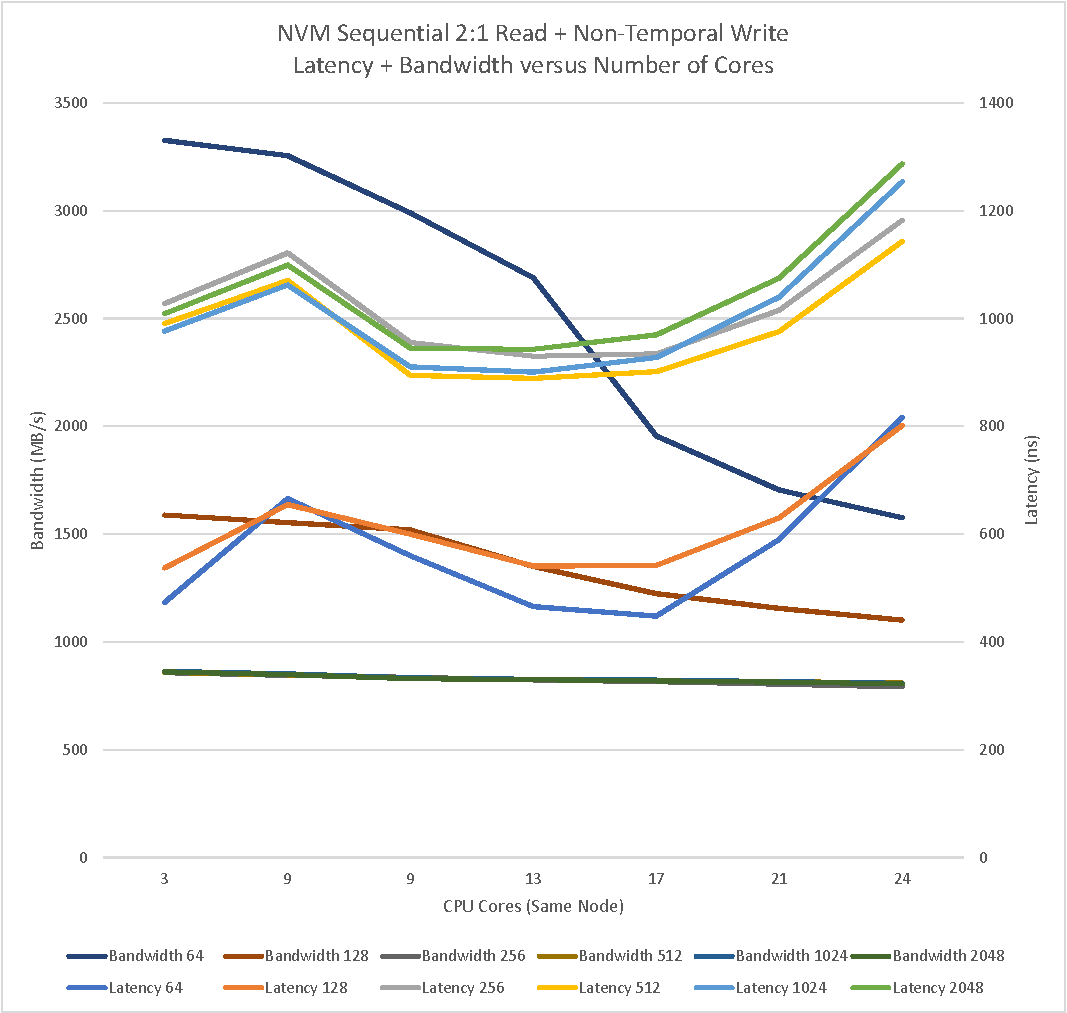
\includegraphics[scale=0.5]{charts/sequential-w7-crop.pdf}
\end{figure}


\begin{figure}
    \centering
    \caption{Sequential 3:1 Read to Non-Temporal Write (streaming triad) (W10)}\label{chart:sequential:W10}
    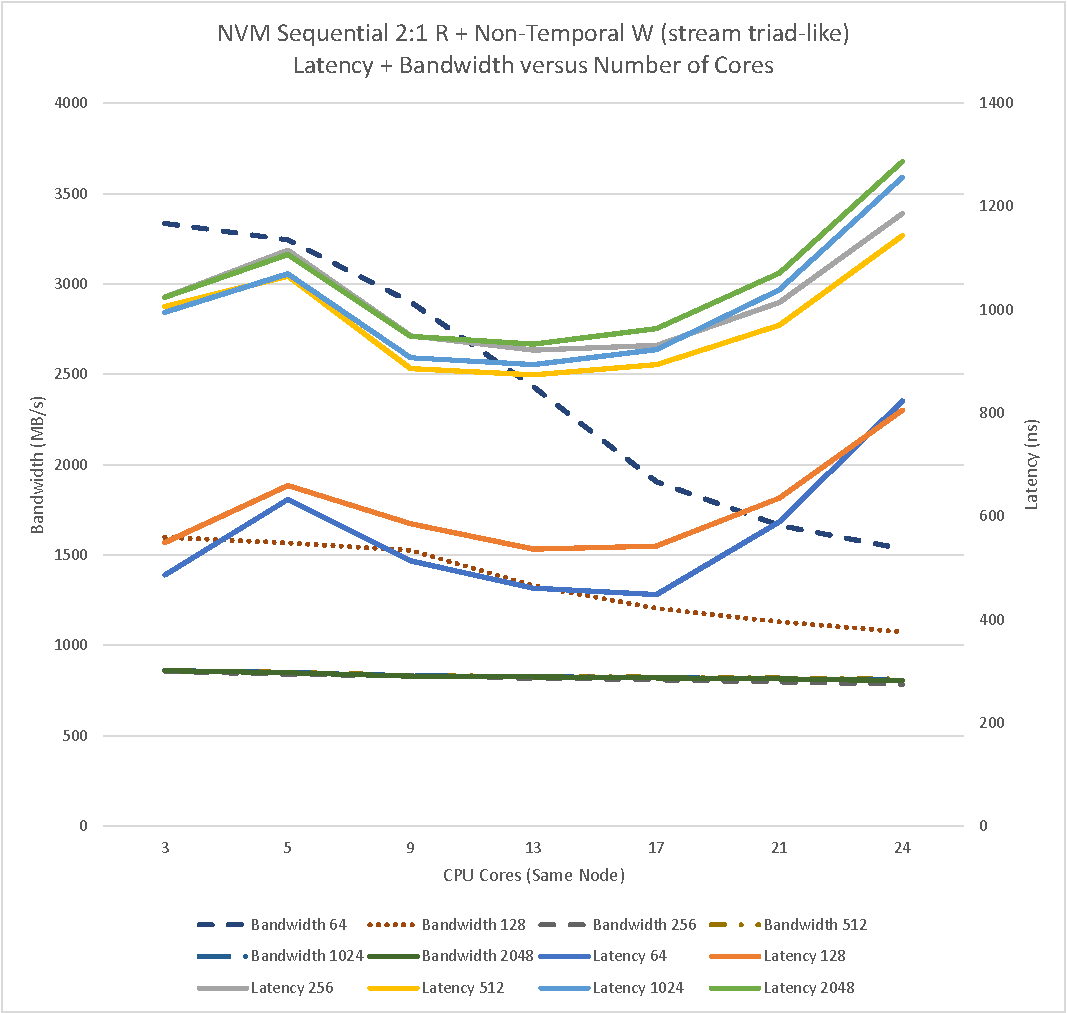
\includegraphics[scale=0.5]{charts/sequential-w10-crop.pdf}
\end{figure}

\endinput



-R read-only load generated, if this is used, -W option should NOT be used 
-Wn where n means
  2  - 2:1 read-write ratio
  3  - 3:1 read-write ratio
  5  - 1:1 read-write ratio
  7  - 2:1 read-Non Temporal Write ratio
  8  - 1:1 read-Non Temporal Write ratio
  10 - 2:1 read-Non Temporal Write ratio (stream triad-like)


dram-baseline-nt-write-same-node.pdf
nt-write-both-nodes.pdf
random-r.pdf
random-W2.pdf
random-W5.pdf
random-w6.pdf
random-W7.pdf
random-W8.pdf
sequential-r.pdf
sequential-w10.pdf
sequential-W2.pdf
sequential-w3.pdf
sequential-W5.pdf
sequential-w6.pdf
sequential-W7.pdf

aep_eval_bandwidth-crop.pdf
aep_eval_idle_latency-crop.pdf
aep_eval_random_read_load_latency-crop.pdf
node-specific-latency-versus-delay-crop.pdf
node-specific-load-data-crop.pdf

